% Appendix Template

\chapter*{Appendix} % Main appendix title

\label{AppendixX} % Change X to a consecutive letter; for referencing this appendix elsewhere, use \ref{AppendixX}

\section{Pseudocode Standard}
\label{appendix:pseudocode-standard}

\quad  Pseudocode is a form of structured English for describing algorithms. It allows designers to focus on algorithmic logic without being distracted by the syntax of a programming language. The pseudocode must be complete, describing the entire logic of an algorithm so that implementation becomes a straightforward translation. The vocabulary used in pseudocode should reflect the problem domain rather than the implementation domain.  

\quad All pseudocode presented in this thesis follows the structured pseudocode style described in this appendix. This standard emphasizes clarity, problem-domain vocabulary, and completeness, ensuring that algorithms are described in a way that is independent of implementation details but precise enough for direct translation into code. The adopted standard is based on the guidelines provided by Dalbey~\cite{dalbey2003pseudocode}.


\subsection{Structured Constructs}
The pseudocode notation is built around six primary constructs:  
\begin{itemize}
	\item \textbf{SEQUENCE}: linear progression of steps.  
	\item \textbf{WHILE}: loop with a test at the beginning.  
	\item \textbf{IF-THEN-ELSE}: binary decision structure.  
	\item \textbf{REPEAT-UNTIL}: loop with a test at the bottom.  
	\item \textbf{CASE}: multiway branching structure.  
	\item \textbf{FOR}: counting loop for iteration.  
\end{itemize}

\quad It has been proven that SEQUENCE, WHILE, and IF-THEN-ELSE are sufficient to implement any algorithm, though the additional constructs simplify common patterns.  

\subsection{Formatting Guidelines}
\quad Sequential control is represented by writing one action per line. Nested constructs must be clearly indented. Common keywords include:  
\begin{itemize}
	\item Input: \texttt{READ, OBTAIN, GET}  
	\item Output: \texttt{PRINT, DISPLAY, SHOW}  
	\item Compute: \texttt{COMPUTE, CALCULATE, DETERMINE}  
	\item Initialize: \texttt{SET, INIT}  
	\item Increment: \texttt{INCREMENT, BUMP}  
\end{itemize}

\quad Subprocedures are invoked using the keyword \texttt{CALL}, and exception handling is represented with \texttt{BEGIN}, \texttt{EXCEPTION}, and \texttt{END}.  

\section{Algorithms}
\label{appendix:supporting-algorithms}

\quad The following algorithms are part of the methods described in the main text. 
Because they are lengthy, they are presented in this appendix to maintain the 
flow of the exposition without interrupting the reader’s focus.


% Algorithm 1: Main Retransmission Manager Loop
\begin{algorithm}
	\caption{Main loop of the Retransmission Manager}
	\label{alg:retransmission-manager}
	\begin{algorithmic}[1]
		\State \textbf{Initialize} phase\_index $\gets 0$, round $\gets 0$
		\While{true}
		\State phase $\gets$ phases[phase\_index]
		\If{phase.enabled = \textbf{false}} 
		\State \textbf{CALL} advance\_phase()
		\State \textbf{Continue} 
		\EndIf
		\State nc\_matrices $\gets$ \textbf{CALL} generate\_nc\_matrices()
		\ForAll{$(m, \mathcal{C}) \in$ nc\_matrices} \Comment{$m$: matrix, $\mathcal{C}$: client list aligned with rows}
		\If{$m$ is empty} \State \textbf{Continue} \EndIf
		\If{phase.mode = Multicast}
		\State already $\gets$ sent\_actions[(phase\_index, round, id($m$))]
		\State actions $\gets$ \textbf{CALL} compute\_retransmissions($m$, already)
		\ForAll{a $\in$ actions}
		\If{\textbf{not} bandwidth\_ok\_multicast(a)} \State \textbf{Continue} \EndIf
		\State sent\_actions[(phase\_index, round, id($m$))] $\gets$ sent\_actions[...] $\cup \{a\}$
		\If{a = Packet($i$)} \State \textbf{CALL} send\_multicast\_packet($i$, $m$) \EndIf
		\If{a = Xor($i,j$)} \State \textbf{CALL} send\_multicast\_xor($i$, $j$, $m$) \EndIf
		\EndFor
		\Else \Comment{Unicast}
		\For{$r \gets 0$ \textbf{to} rows($m$)$-1$}
		\State client $\gets \mathcal{C}[r]$; missing $\gets$ \textbf{CALL} row\_missing($m$, r)
		\ForAll{$i \in$ missing}
		\If{\textbf{not} can\_send\_this\_round(phase\_index, round, client, i)} \State \textbf{Continue} \EndIf
		\If{\textbf{not} bandwidth\_ok\_unicast(client)} \State \textbf{Break} \EndIf
		\State sent\_actions[(phase\_index, round, client, i)] $\gets$ Packet($i$)
		\State \textbf{CALL} send\_unicast\_packet($i$, client)
		\EndFor
		\EndFor
		\EndIf
		\EndFor
		\State \textbf{CALL} advance\_phase()
		\State round $\gets$ round $+$ 1
		\EndWhile
	\end{algorithmic}
\end{algorithm}

% Algorithm 2: Greedy Action Selection with Coding
\begin{algorithm}
	\caption{Greedy action selection with coding in compute\_retransmissions}
	\label{alg:compute-retransmissions}
	\begin{algorithmic}[1]
		\State $R \gets$ rows($m$), $P \gets$ cols($m$)
		\State missing\_count[$0..P-1$] $\gets 0$
		\For{$i \gets 0$ \textbf{to} $P-1$} 
		\State missing\_count[$i$] $\gets$ number of rows $r$ with $m[r,i]=0$ 
		\EndFor
		\State needed $\gets \{i \mid$ missing\_count[$i$]$>0 \land$ Packet($i$) $\notin$ already$\}$
		\If{needed is empty} \State \Return $[]$ \EndIf
		\State best\_xor $\gets$ None; gain $\gets 0$
		\For{$i \gets 0$ \textbf{to} $P-1$}
		\If{missing\_count[$i$]$=0$} \State \textbf{Continue} \EndIf
		\For{$j \gets i+1$ \textbf{to} $P-1$}
		\If{missing\_count[$j$]$=0$ \textbf{or} Xor($i,j$)$\in$already} \State \textbf{Continue} \EndIf
		\State $b \gets$ number of rows $r$ with $(m[r,i] \oplus m[r,j])=1$
		\If{$b >$ gain} \State gain $\gets b$; best\_xor $\gets (i,j)$ \EndIf
		\EndFor
		\EndFor
		\State needed\_sorted $\gets$ needed sorted by missing\_count descending
		\State actions $\gets$ first $K$ elements of $\{\text{Packet}(i) \mid i \in$ needed\_sorted$\}$ with $K=5$
		\If{best\_xor $\neq$ None and gain $>$ missing\_count[needed\_sorted[0]]}
		\State remove head of actions if nonempty
		\State prepend Xor(best\_xor) to actions
		\EndIf
		\State \Return actions
	\end{algorithmic}
\end{algorithm}

% Algorithm 3: NC Matrix Construction from Client Reports
\begin{algorithm}
	\caption{Construction of NC matrices from client reports}
	\label{alg:generate-nc-matrices}
	\begin{algorithmic}[1]
		\State nc\_maps $\gets$ empty map from matrix\_id to (matrix, client\_list)
		\ForAll{client $\in$ clients}
		\ForAll{report $\in$ client.reports}
		\State id $\gets$ report.matrix\_index; bm $\gets$ report.bitmap
		\If{id $\notin$ nc\_maps} \State nc\_maps[id] $\gets$ (empty\_matrix, empty\_list) \EndIf
		\State append bm as new row to nc\_maps[id].matrix
		\State append (client.client\_id, client.ip) to nc\_maps[id].client\_list
		\EndFor
		\EndFor
		\State \Return nc\_maps
	\end{algorithmic}
\end{algorithm}


\section{Evaluation Appendix}
\label{appendix:evaluation appendix}

\begin{figure}[H]
	\centering
	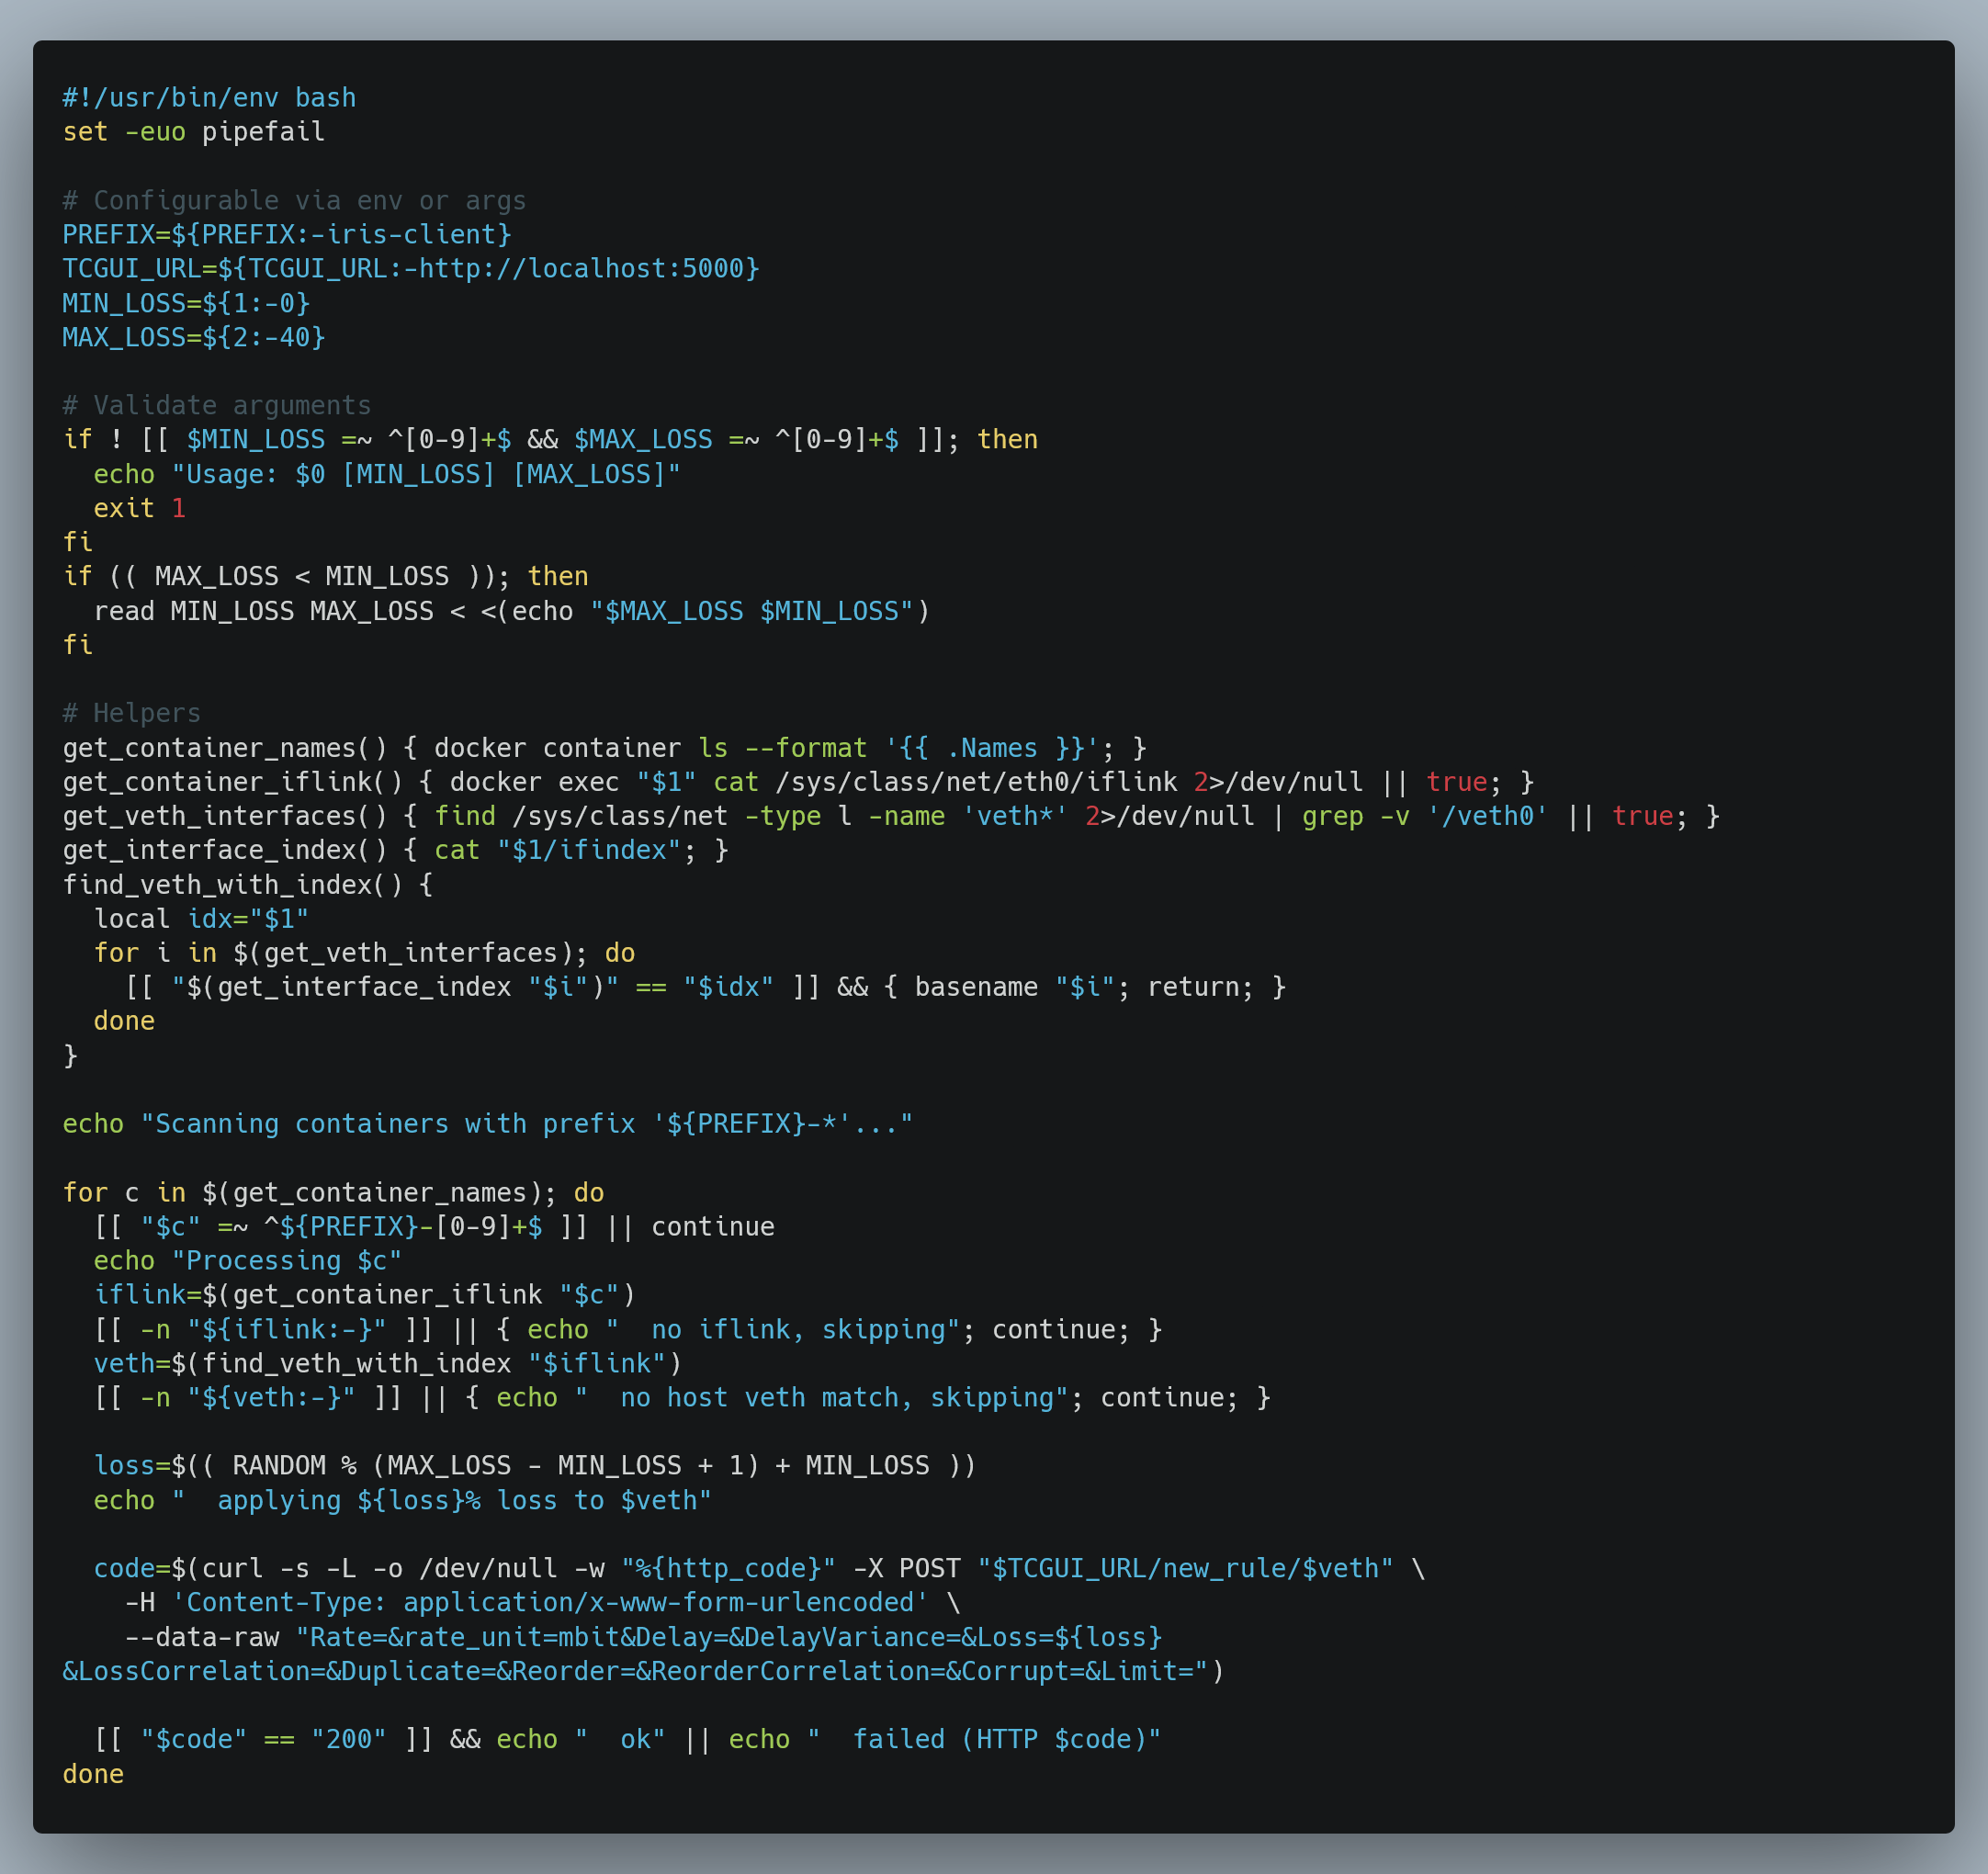
\includegraphics[width=1\textwidth]{Appendix/packet_loss_script.png}
	\caption{Script to apply random packet loss to containers}
	\label{fig:random loss script}
\end{figure}


\begin{figure}[H]
	\centering
	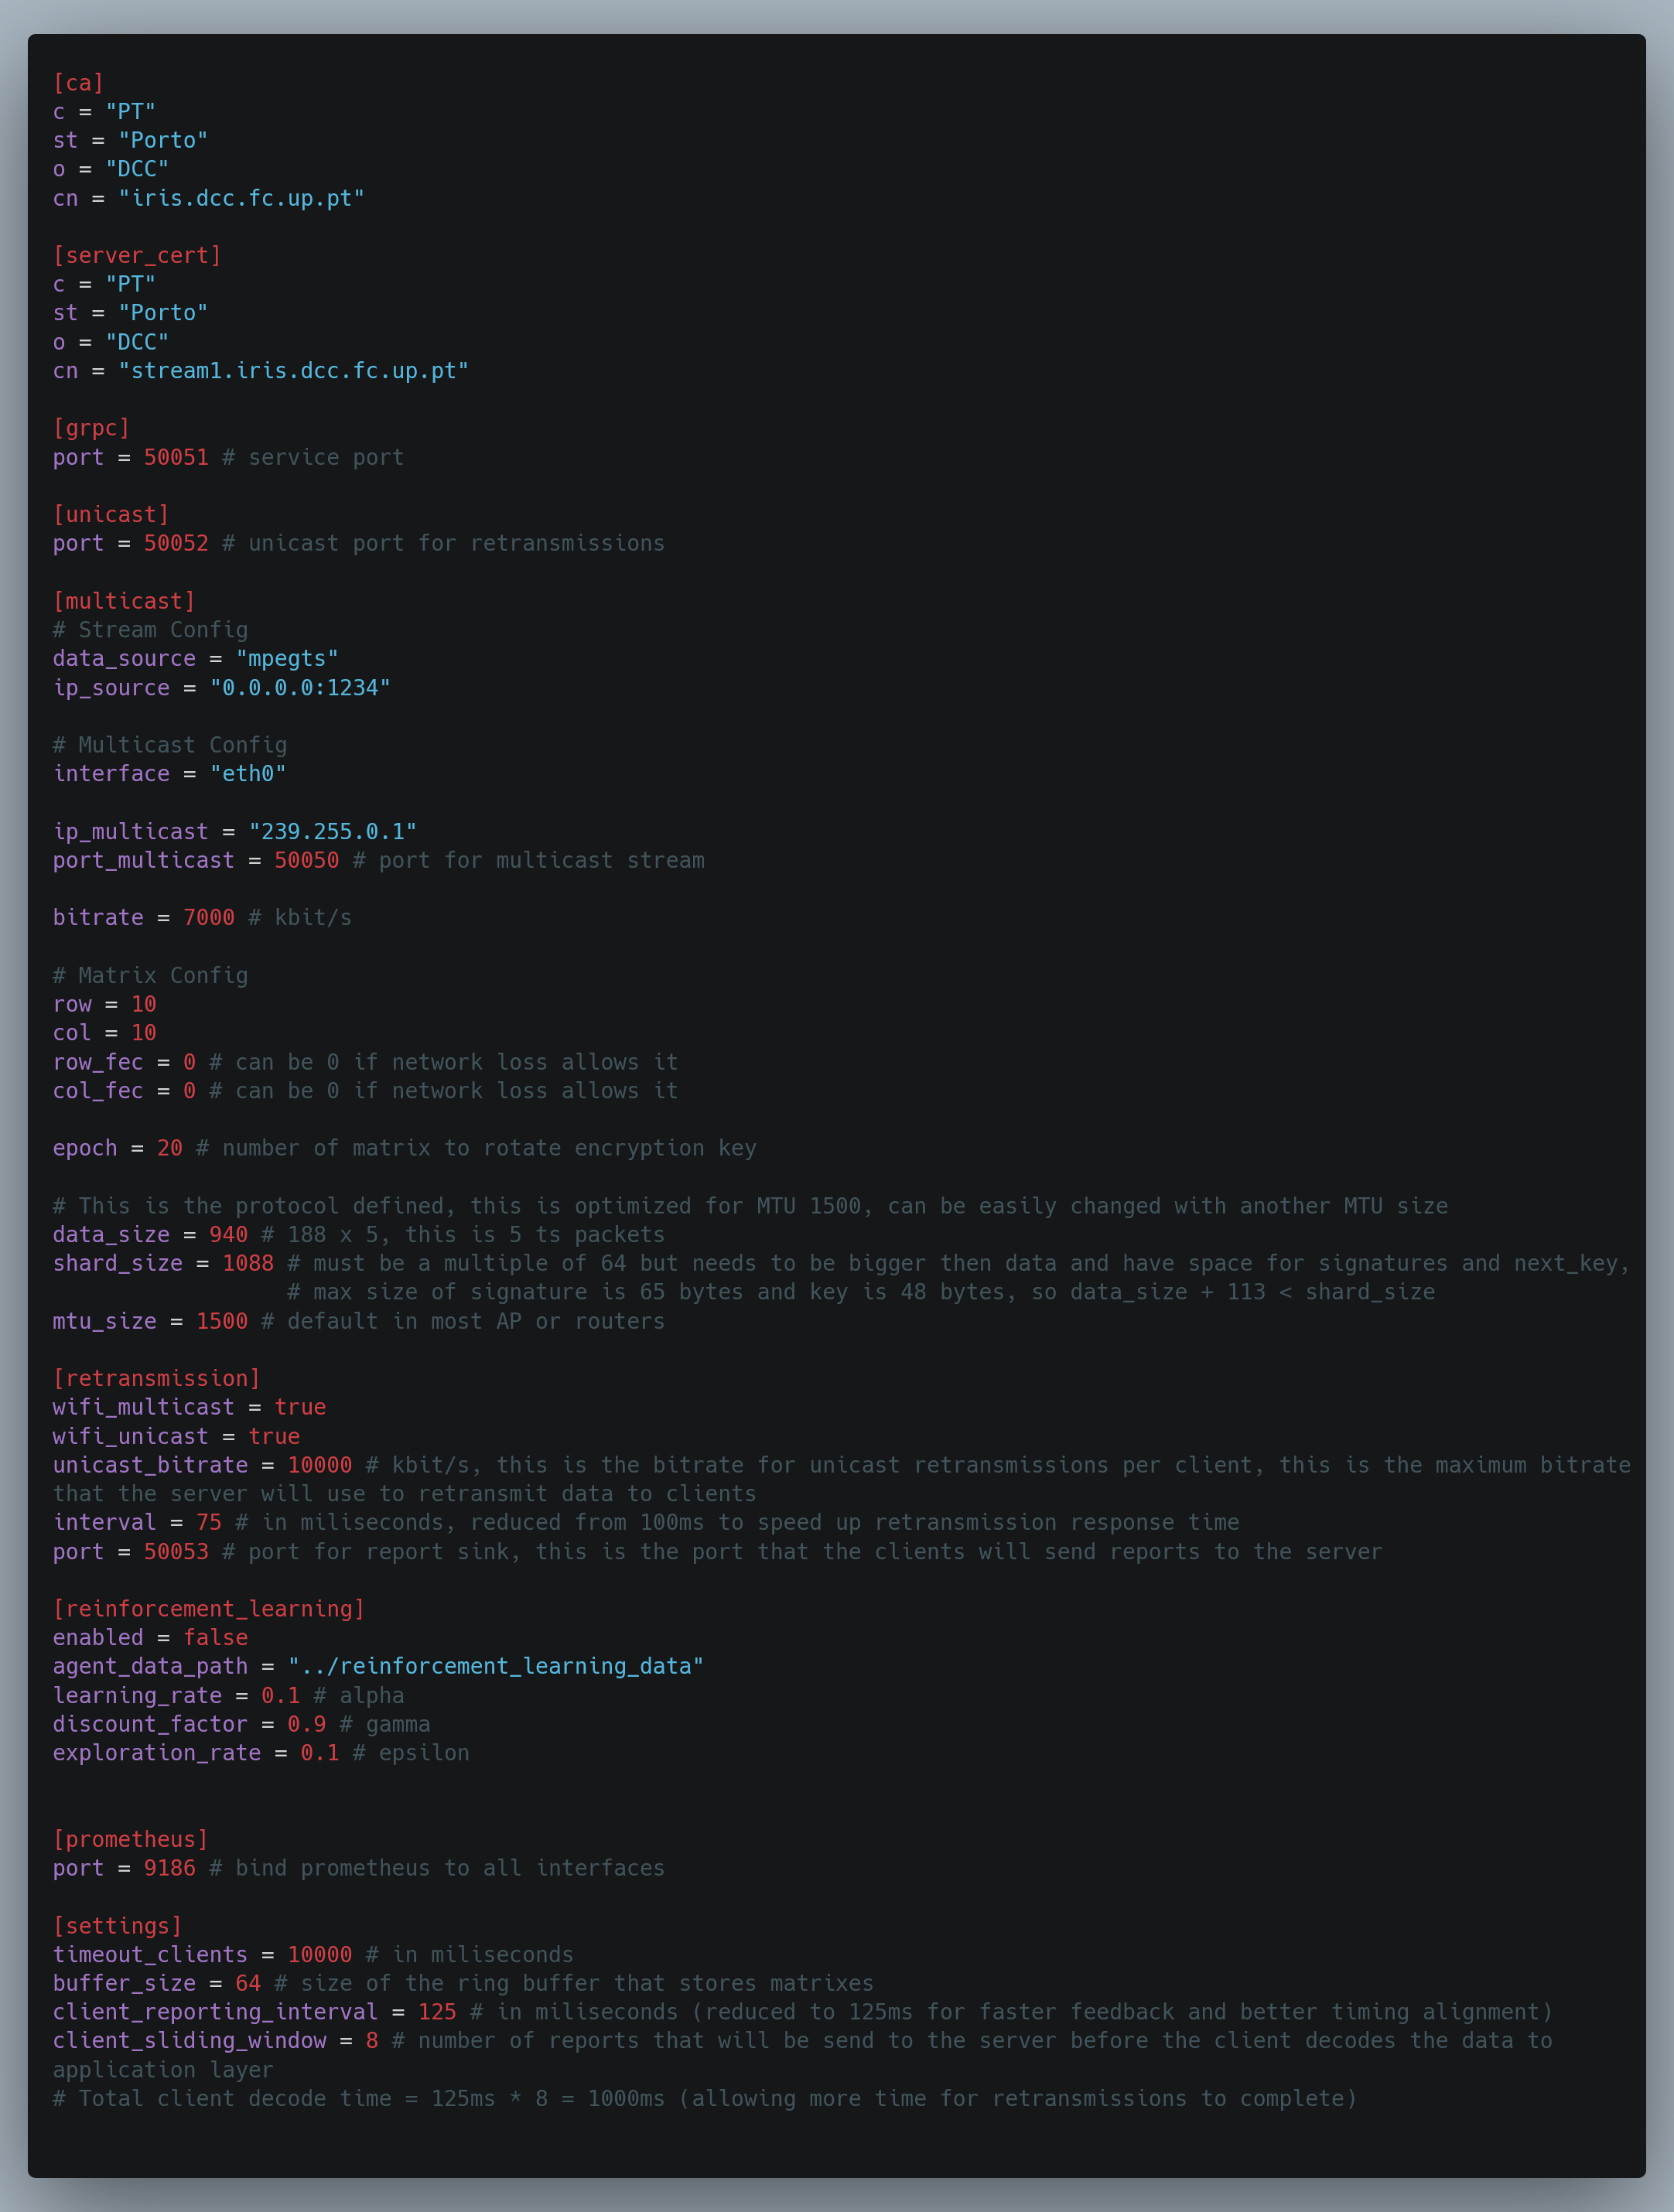
\includegraphics[width=1\textwidth]{Appendix/server_config.png}
	\caption{Server config example}
	\label{fig:server config}
\end{figure}

\begin{figure}[H]
	\centering
	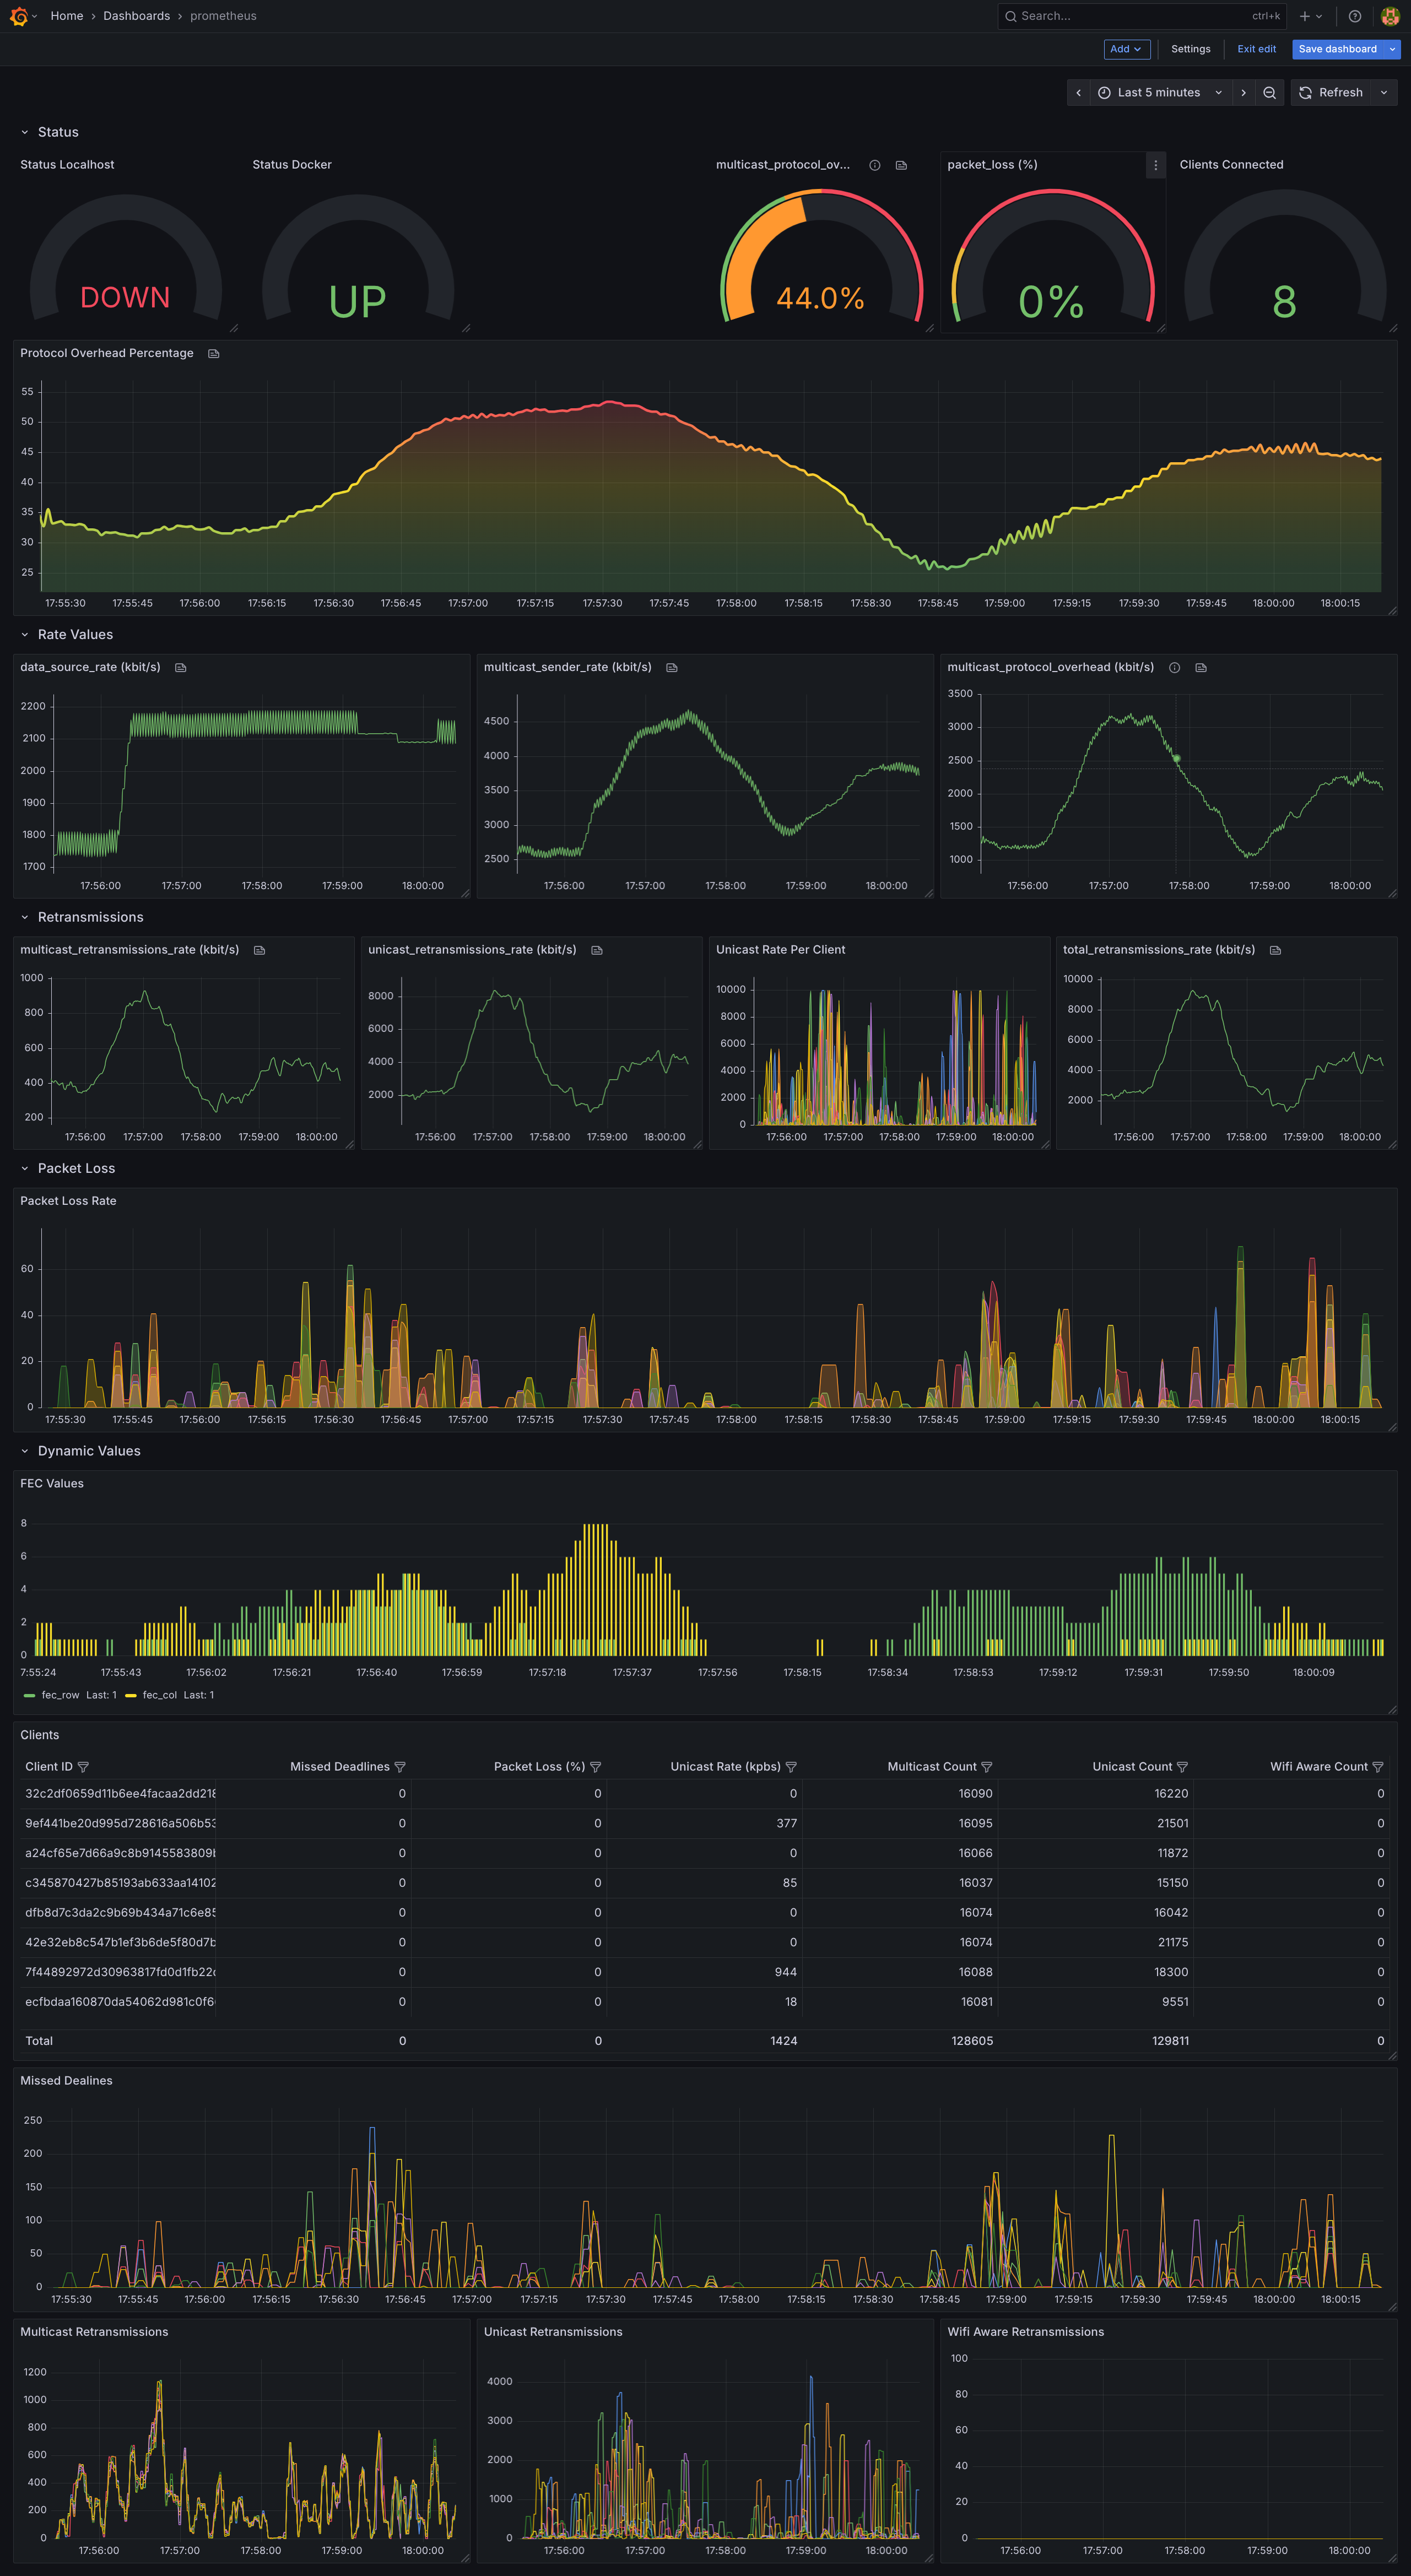
\includegraphics[width=0.9\textwidth]{Appendix/baseline.png}
	\caption{Grafana dashboard from one scenario}
	\label{fig:grafana dashboard}
\end{figure}
